\documentclass[12pt]{article}
\usepackage[T1]{fontenc}
\usepackage[utf8]{inputenc}
\renewcommand*\familydefault{\sfdefault}

\usepackage{anysize}
\marginsize{2.5cm}{2.5cm}{1cm}{1.5cm}
\setlength{\marginparwidth}{2cm}

% \usepackage{authblk}
\usepackage{graphicx}
\usepackage{import} 
\usepackage{subfig}
\graphicspath{{../../results/}}

\usepackage{xcolor}

\usepackage[font=small,labelfont=bf]{caption}

\def\labelitemi{--}

% Line numbers
\usepackage[left]{lineno}
%\linenumbers

\usepackage[color=red!60]{todonotes}

\usepackage{pgfplotstable}
\pgfplotsset{compat=1.16}
\def\getcell#1#2#3{
\pgfplotstablegetelem{#1}{[index]#2}\of{#3}\pgfplotsretval%
}

% Tables 
\pgfplotstableset{col sep=tab, header=has colnames, string type, text special chars={\%}} 
\pgfplotstableread{../../results/201030_europe3_table01.tsv}{\casestable}
\pgfplotstableread{../../results/201030_europe3_table02.tsv}{\firsttable}


\title{A comprehensive study of the early phylodynamics of SARS-CoV-2 in Europe}


\begin{document}
\maketitle

\begin{abstract}
\todo[inline]{TODO abstract}
This project focus on the spatial dynamics of the early spread of SARS-CoV-2 in Europe. We apply a novel approach based on the Multi-type Birth Death phylodynamic model to infer structured population dynamics jointly with between-subpopulation transmission rates from viral genome sequences. The inferred epidemic trajectories for the combined outbreak responsible for the observed sequence data will allow us to better understand the entry into and early spread of SARS-CoV-2 in Europe.

% The early dynamics of the epidemic in Europe surprised the whole world/ From isolated cases detexcted in some, ina  few weeks we faced an unprecedent epidemic with case numbers and death counts stressing well stalished health infraestructures. Understanding what happened during those first month could prepare us to be less surpred in similar future events. Complex dynamics, typical epi date, case identification and travel history, very likely not all cases reported. Genetic sequences are a valuable source of information than together with popualtion dynamic model could inform us about the firrst steps of the coronavirus in Europe. We have integrated sequence data, flisht data and bayesian inference priors? to infer population trajectories - case counts and migration dynamics between the most relevant countrries at the start of the European pandemic.
\end{abstract}


\section*{Introduction}
\todo[inline]{TODO introduction}

\begin{itemize}
\item Importance of understanding the spread of the virus to prevent future outbreaks 

\item About phylodynamics/phylogeographics? Use of genetic sequences as a source of information combined with other sources of information as travel data

\item About what we know of the introduction of sars-cov-2 in Europe and early dynamics till 8 March

\item About what we know of the case counts in Europe? Can sequences help?

\item Introduce/formulate the questions: case counts, first introductions, ?migration vs within region transmission?, migration patterns, ?border closures.
\end{itemize}

\section*{Results}
% \todo{Modify tables in R to have one value per cell, nr rate and times}

\todo[inline]{The figures are from analysis Europe3: subsampled datasets according to cases/day and constant migration rate (no GLM), same xml specifications than Sarah's analysis.}

\subsubsection*{Burden of SARS-CoV-2 infections in Europe}

The inferred epidemic trajectories contain the information about the total number of cases until 8th of March. For the European countries, we obtain an inferred number of total cases above the number of confirmed cases to ECDC, consistent with known limited test availability of the first wave and  previous studies results \cite{Li2020} \cite{Wu2020}. These cases counts correspond to \todo{Include values} x-y times higher than the number of reported cases. Italy is the country with the highest infered number of cases x, followed by Spain, France and Germany. The infered number of cases for China is below the reported number of cases. \todo{limitations of the model, sequence information, partial outbreak dynamics}\\


\begin{figure}[ht]
    \centering
    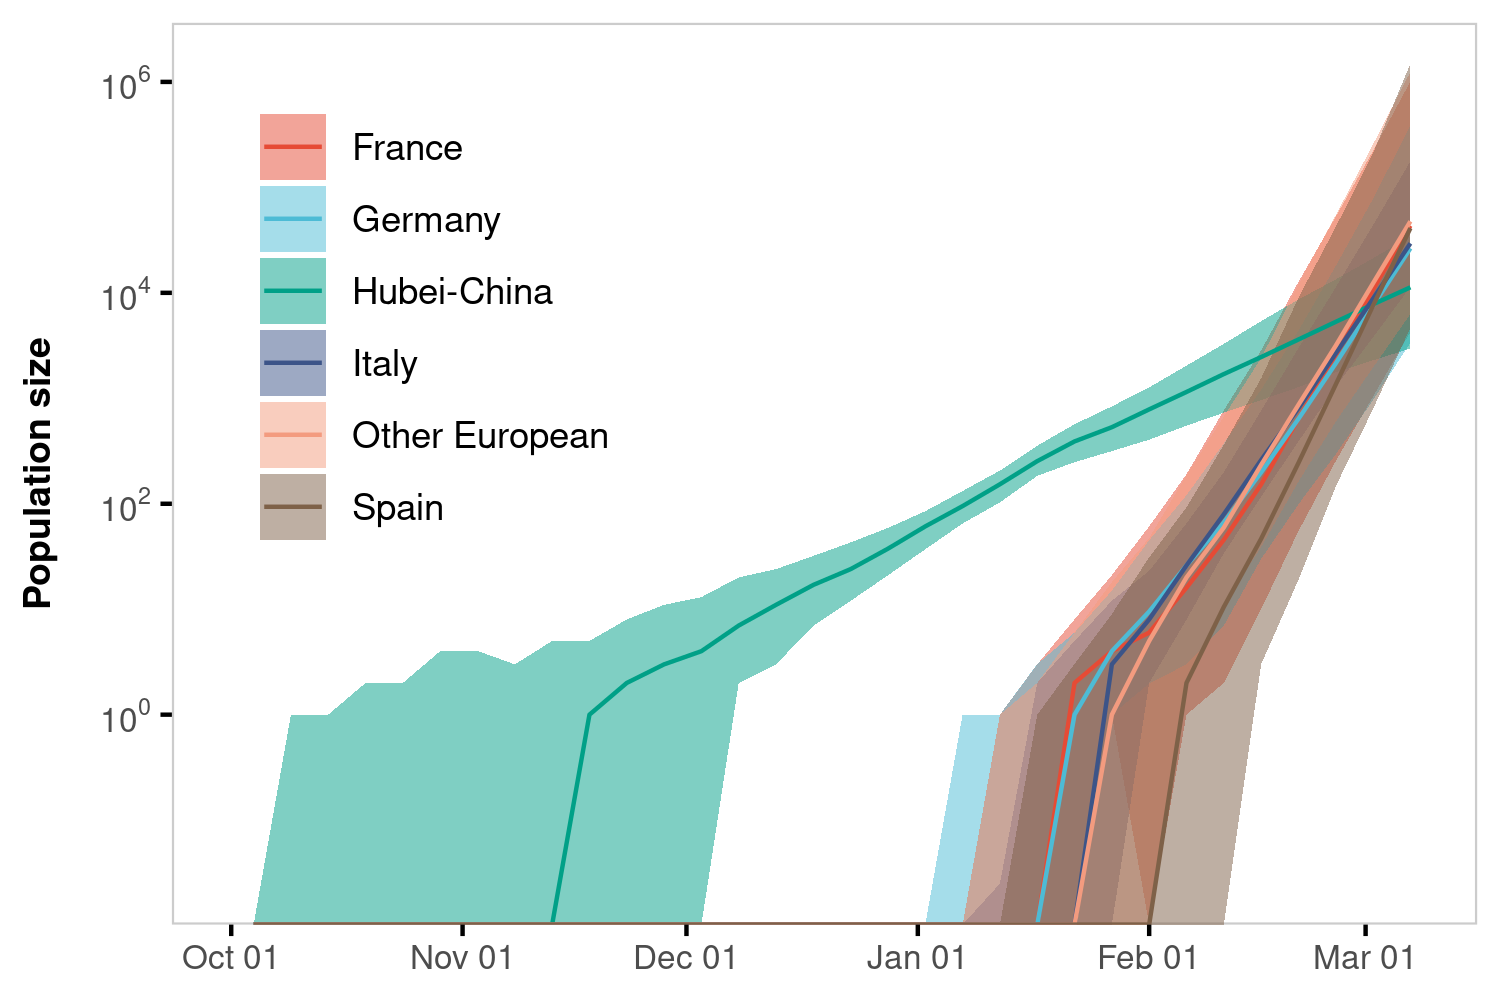
\includegraphics[width=0.8\textwidth]{201030_europe3_figtraj01.png}
    \caption{Inferred population size summary statistics for each deme over time. The line represents the median population trajectory and the interval is the 95\%  credible interval in log scale from a random subsampled set of inferred epidemic trajectories.}
    \label{fig:gribbon}
\end{figure}


\begin{figure}[p]
    \centering
    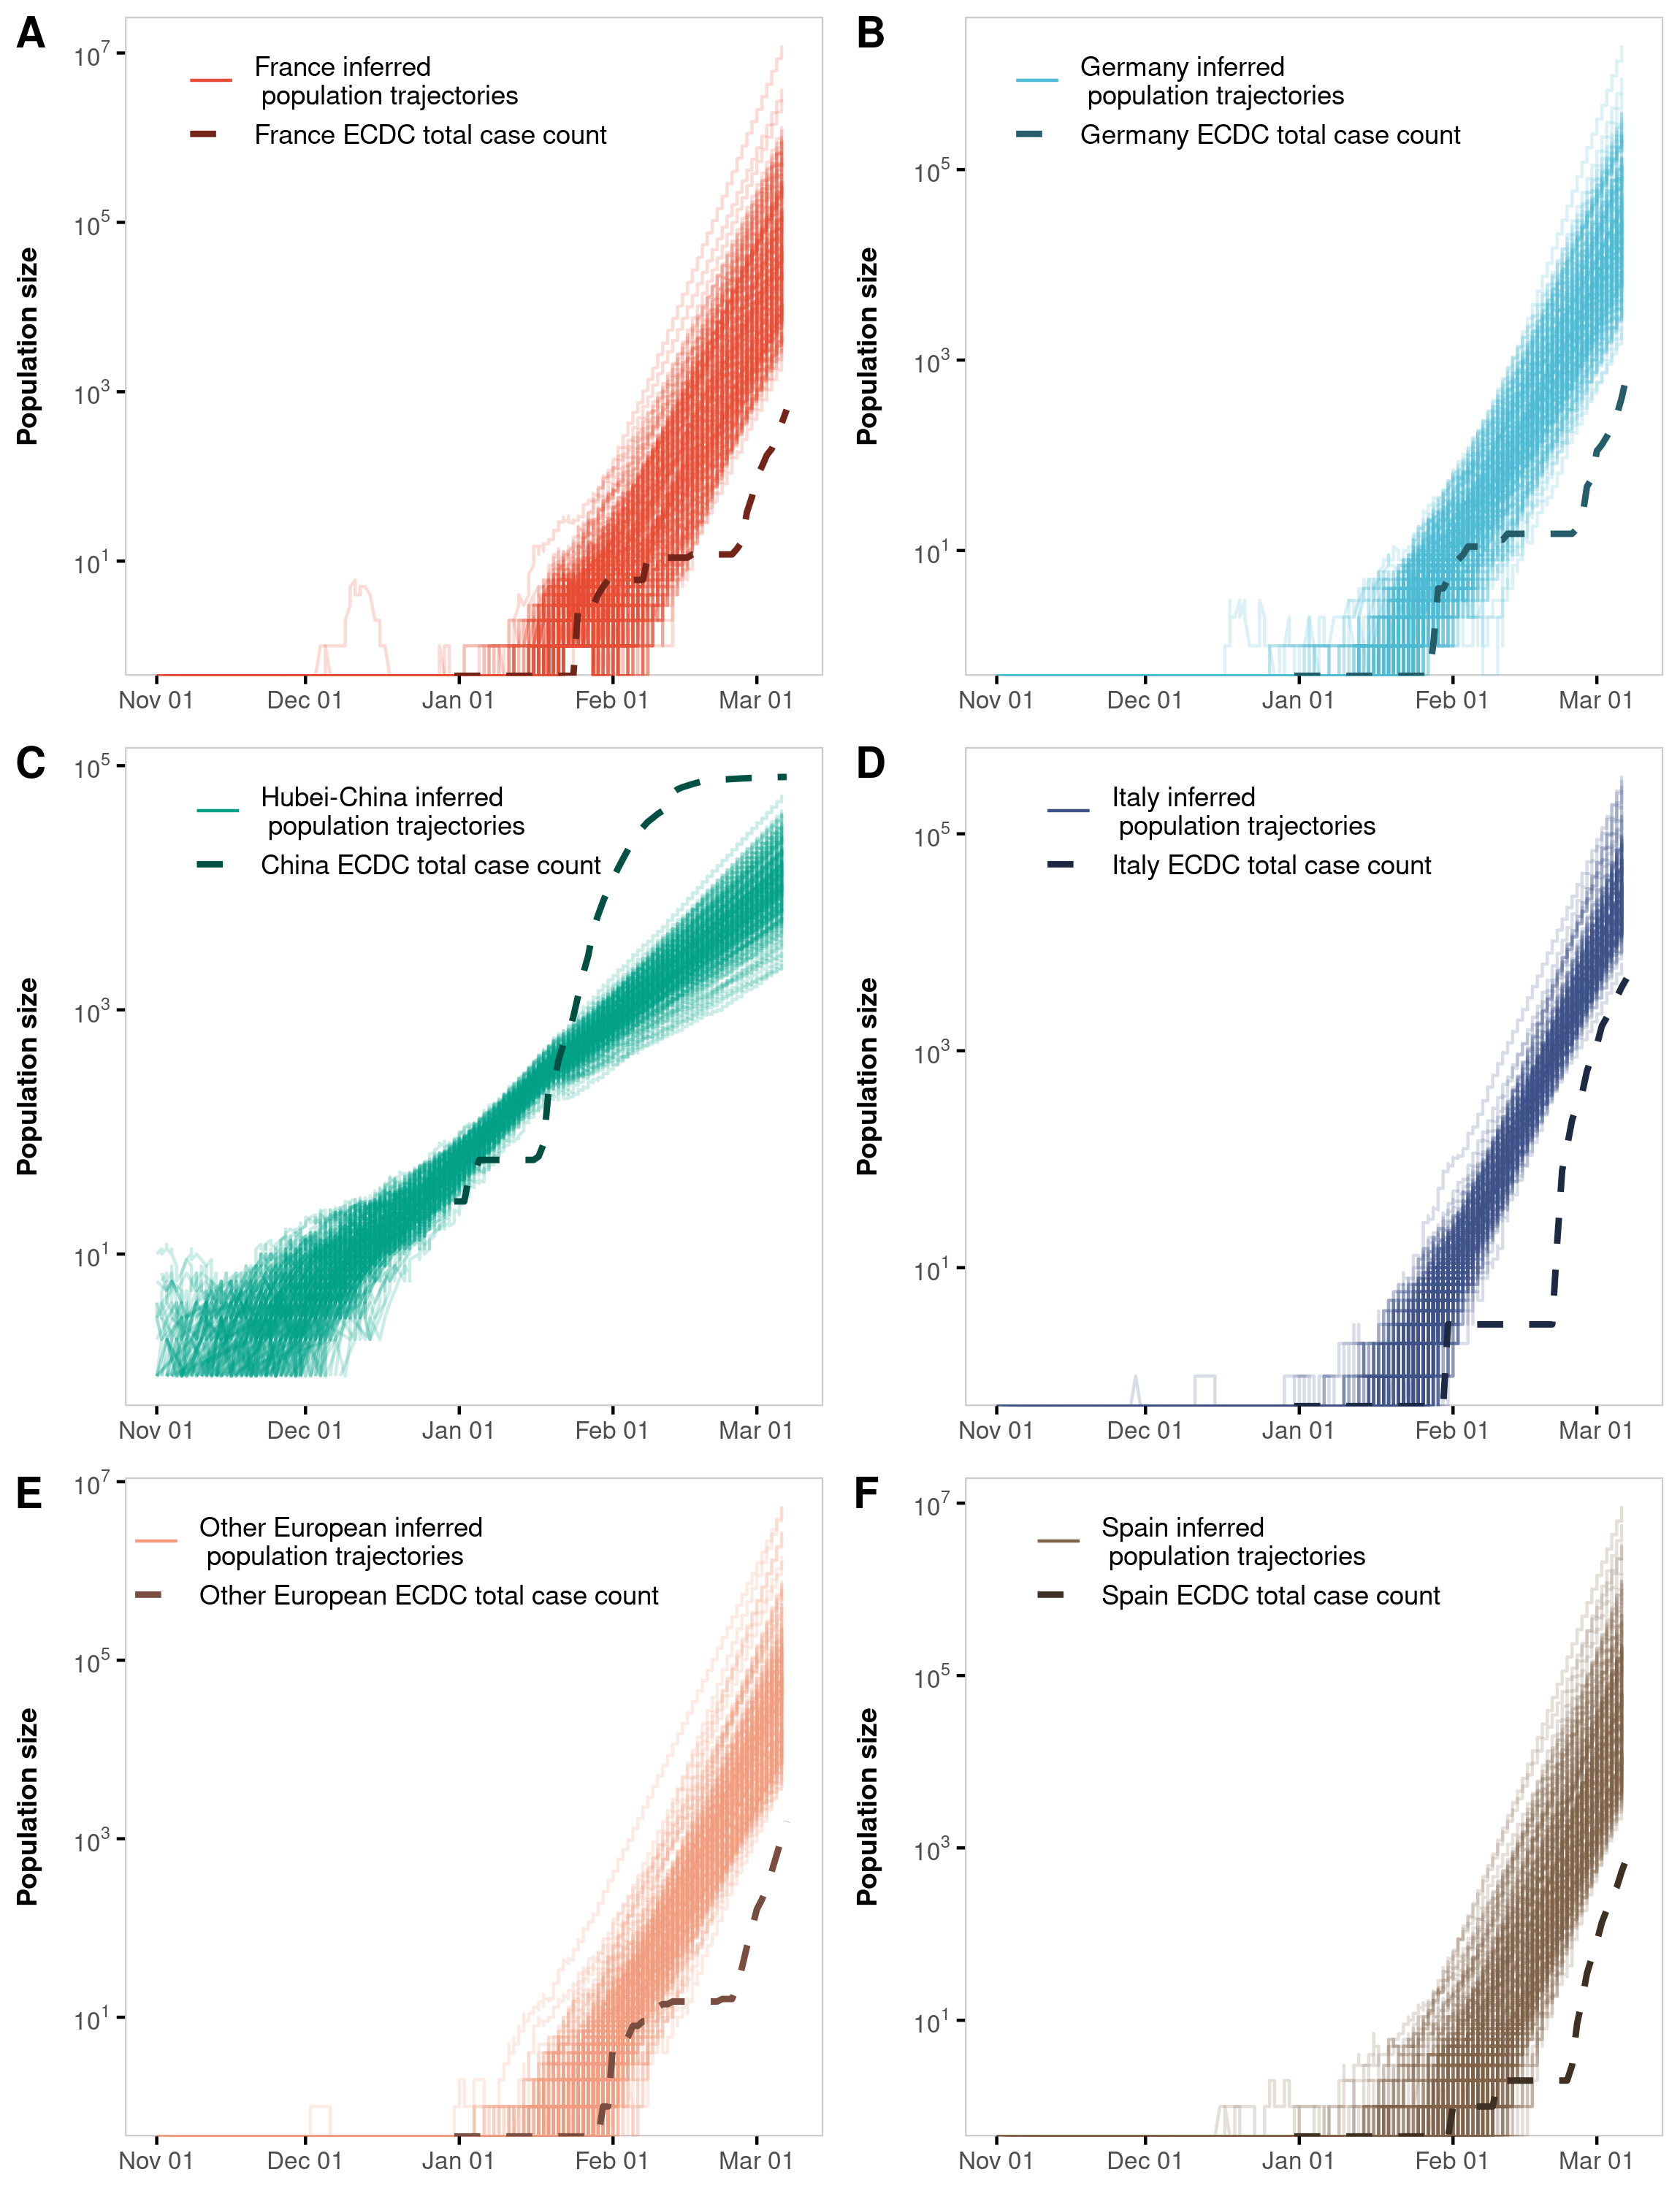
\includegraphics[width=0.9\textwidth]{201030_europe3_figtraj02.png}
    \caption{Inferred epidemic trajectories over time. A random subsampled set of 500 trajectories is plotted. In each subplot, the trajectories (solid lines) are compared with the ECDC cumulative case count data (dashed line) in log scale.}
    \label{fig:trajs}
\end{figure}


In Figure \ref{fig:gribbon} and/or \ref{fig:trajs} we compare the total number of inferred cases by day to the total cumulative number of cases that have been reported to ECDC that same day. Our inferred case counts follow a exponential growth earlier in time than the reported curve and with higher number of cases, being the difference bigger for later times in the epidemic.\\


\begin{figure}[ht]
    \centering
    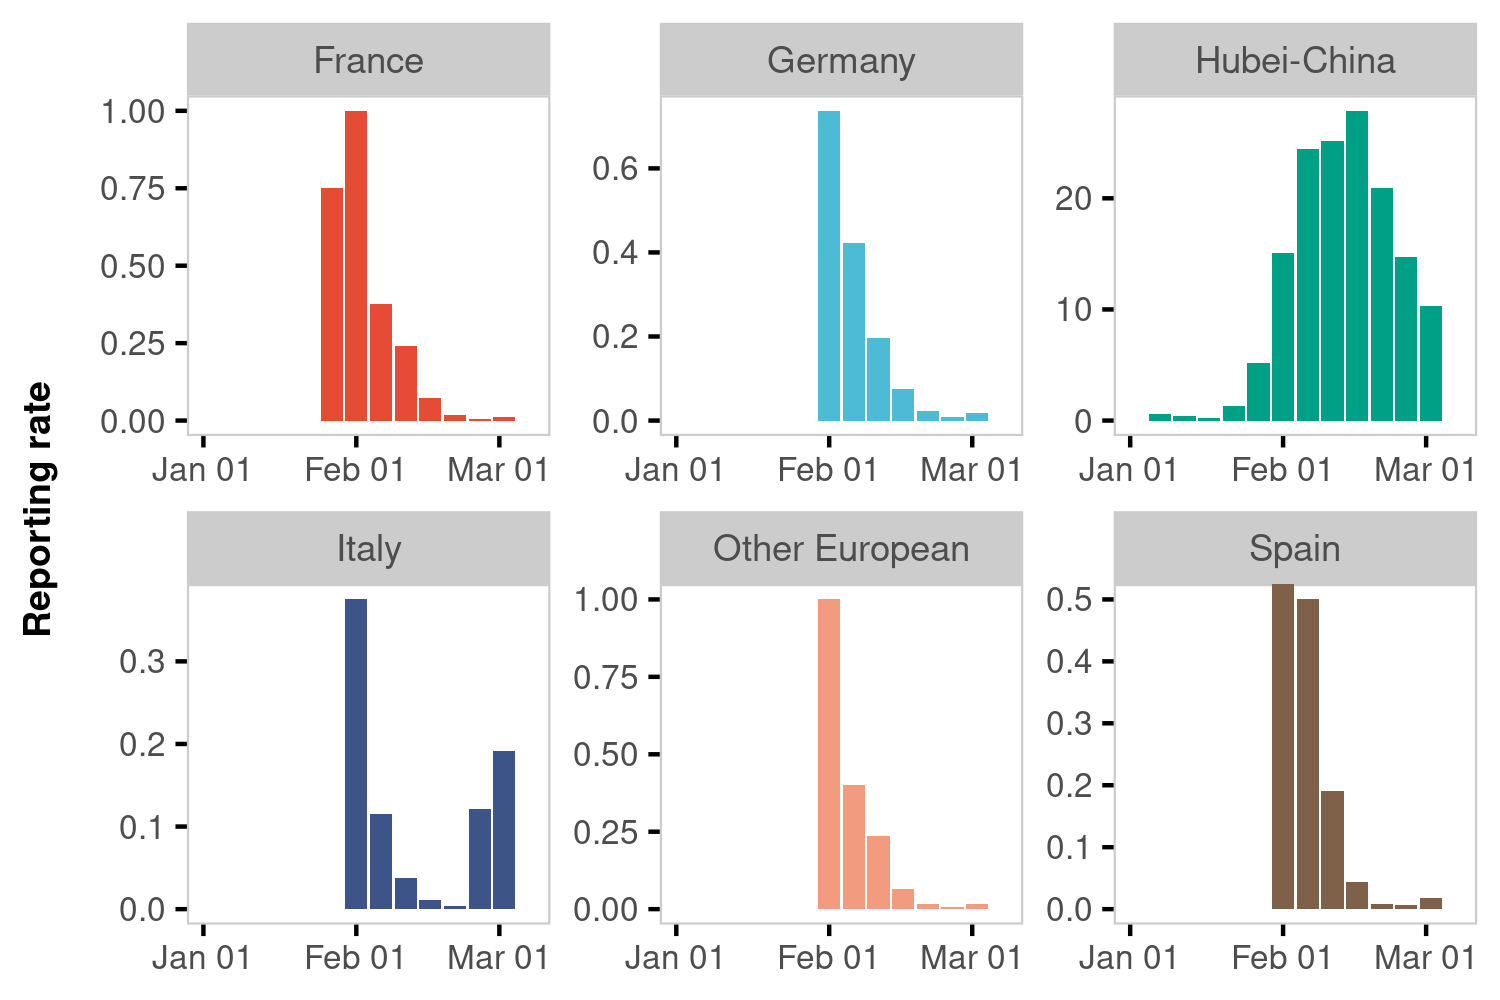
\includegraphics[width=0.9\textwidth]{201030_europe3_figtraj03.png}
    \caption{5-days reporting rate, calculated as the cumulative number of ECDC reported cases by the median number of cumulative inferred cases in intervals of 5 days until 8th of March. }
    \label{fig:reported}
\end{figure}

We can think of a reporting rate as the number of reported cases relative to the total number of cases inferred by the model. This reporting rate decreases with time for all European countries, except for Italy that increases again around March, Figure \ref{fig:reported}. 


\subsubsection*{First introductions into European countries}

\begin{figure}[p]
    \centering
    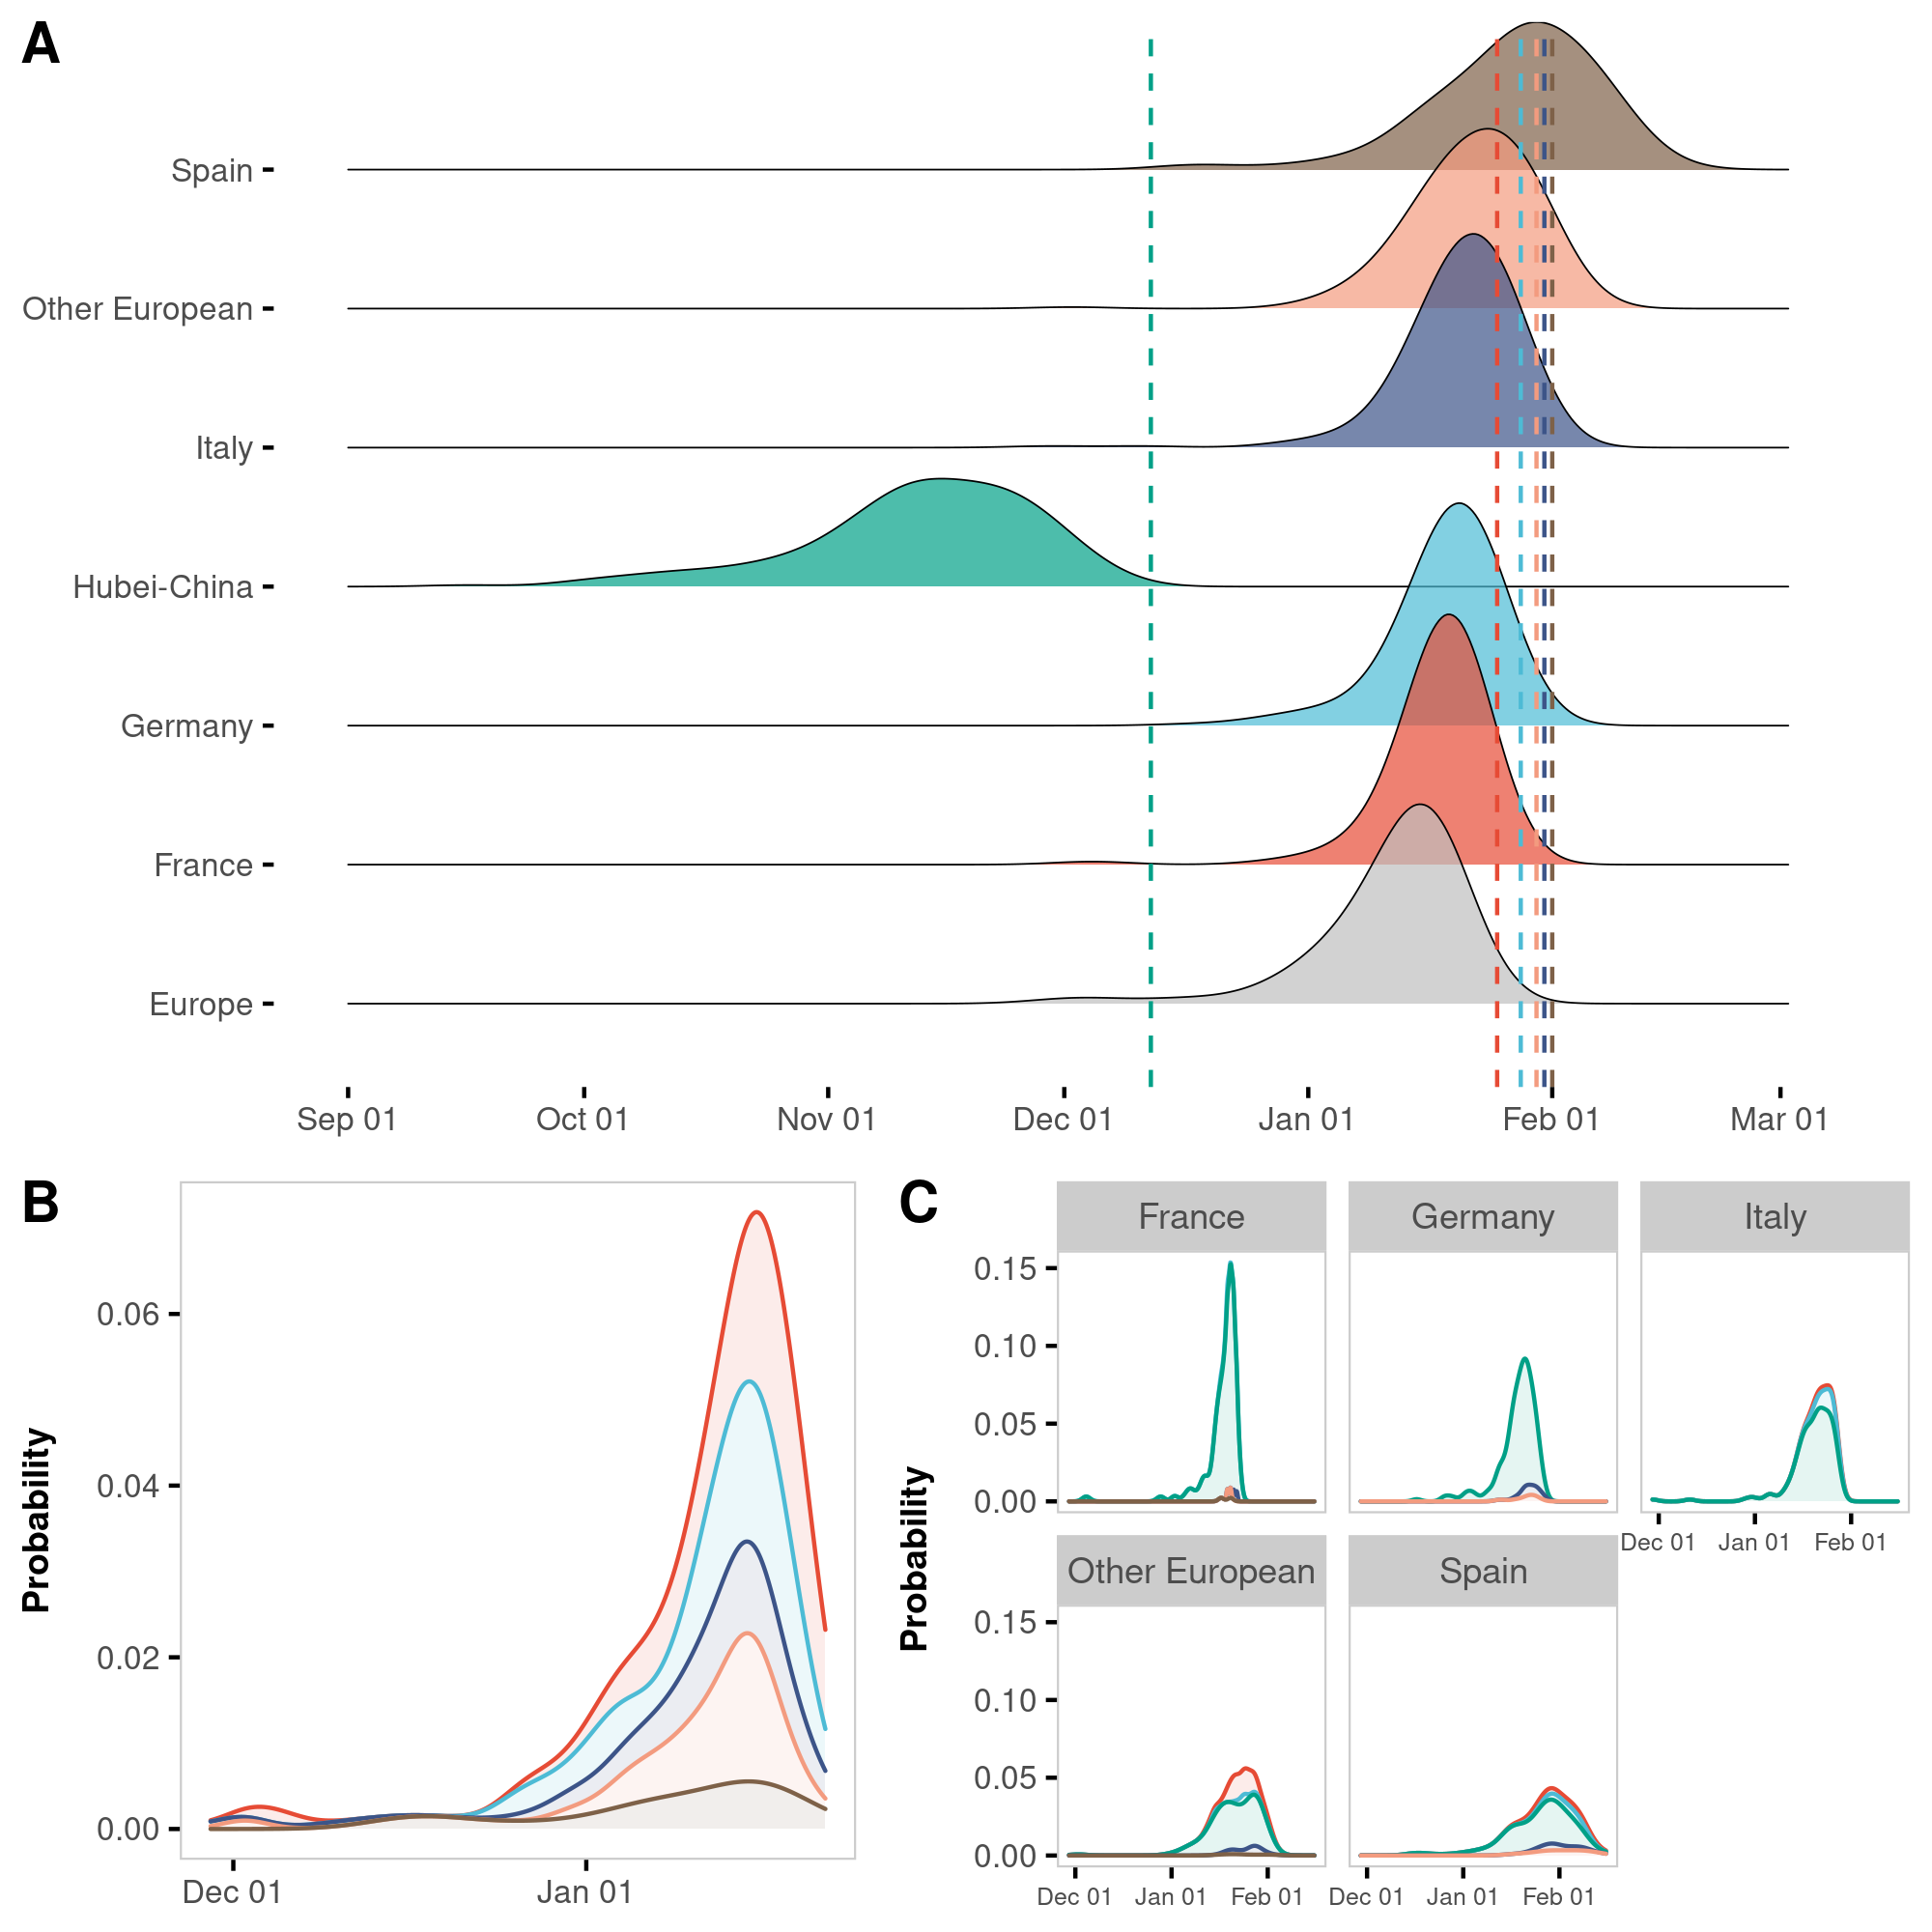
\includegraphics[width=\textwidth]{201030_europe3_figtraj04.png}
    \caption{First introductions of SARS-CoV-2. From the set of random subsampled trajectories, the first introduction time for each epidemic trajectory is recorded and the probability distribution over all these times is plotted. \textbf{A} Probability density of the time of first introduction for each deme. Each dotted line represents the first date when cases where reported to ECDC by deme color. In the case of China, the distribution of the origin time is plotted, since in the analysis we defined Chine as the origin of the epidemic with probability 1. For the other five demes, the distribution of the time of first migration into the deme is shown. \textbf{B} Stacked probability density of the destination of first introduction into Europe coloured by the destination deme. This first case corresponds to the first migration event from China to any of the European countries. \textbf{C} Stacked probability density of the source of the first introduction for each deme coloured by the source deme of the introduction.}
    \label{fig:first}
    \todo[inline]{ticks for every month}
\end{figure}

We would like to answer the question of when and where the first case in Europe occured. We can look to the model inferred epidemic trajectories and analyze the time distribution of the first case in Europe and in each deme. China is defined as the origin of the epidemic in the analysis and this is reflected in Figure \ref{fig:first} A. The occurrence of the origin of the epidemic, i.e. first case in China, is almost one month before the epidemic starts in any European country, ranging \todo{Include values}  x-y. The inferred date of the first case in Europe is inferred to be between a 95\% interval x-y. Among the European countries, France and Germany have the earlier time of introduction, followed by Italy, Other European deme and Spain. We can compare this inferred dates of introduction with the day each country reported its first case to ECDC. In all cases, the reported day was later than the median of the inferred distribution, but it is inside the 95\% interval.\\

The first case in Europe for each trajectoy corresponds to a migration from China to any European country. We can analyze the destination of this first migration into Europe as is shown in Figure \ref{fig:first} B. According to our model, the probability that this first European case was in Spain is very low. The destination of the first case amonth the rest of European demes is equally probable and there is no clear difference in the time distribution for each destination country, with a maximum probability around x.\\
\todo{explain this better, compute the probability of the first case in Europe destination}

The first case in each European country could have been imported from China or from other European country with an ongoing epidemic that started earlier. However, in our analysis we obtain a much higher support for China being the most probable source of the first case for all European demes, Figure \ref{fig:first} C.\\

Even if the first case in each European country came from China, the timing of the introductions in the European countries relative to each other probablu expanded across several days, defining and order of countries with the time of their first case. 

We can analyze if this order of countries, defined by the time in which the first case occured, is shared among the majority of the inferred population trajectories, Figure \ref{fig:first_imig}. We obtain that the first European country with a SARS-CoV-2 case was more likely France or Germany, followed by Italy and Other European deme. While Spain was more likely the last European country with a case among the ones included in the analysis.\\

\begin{figure}[ht]
    \centering
    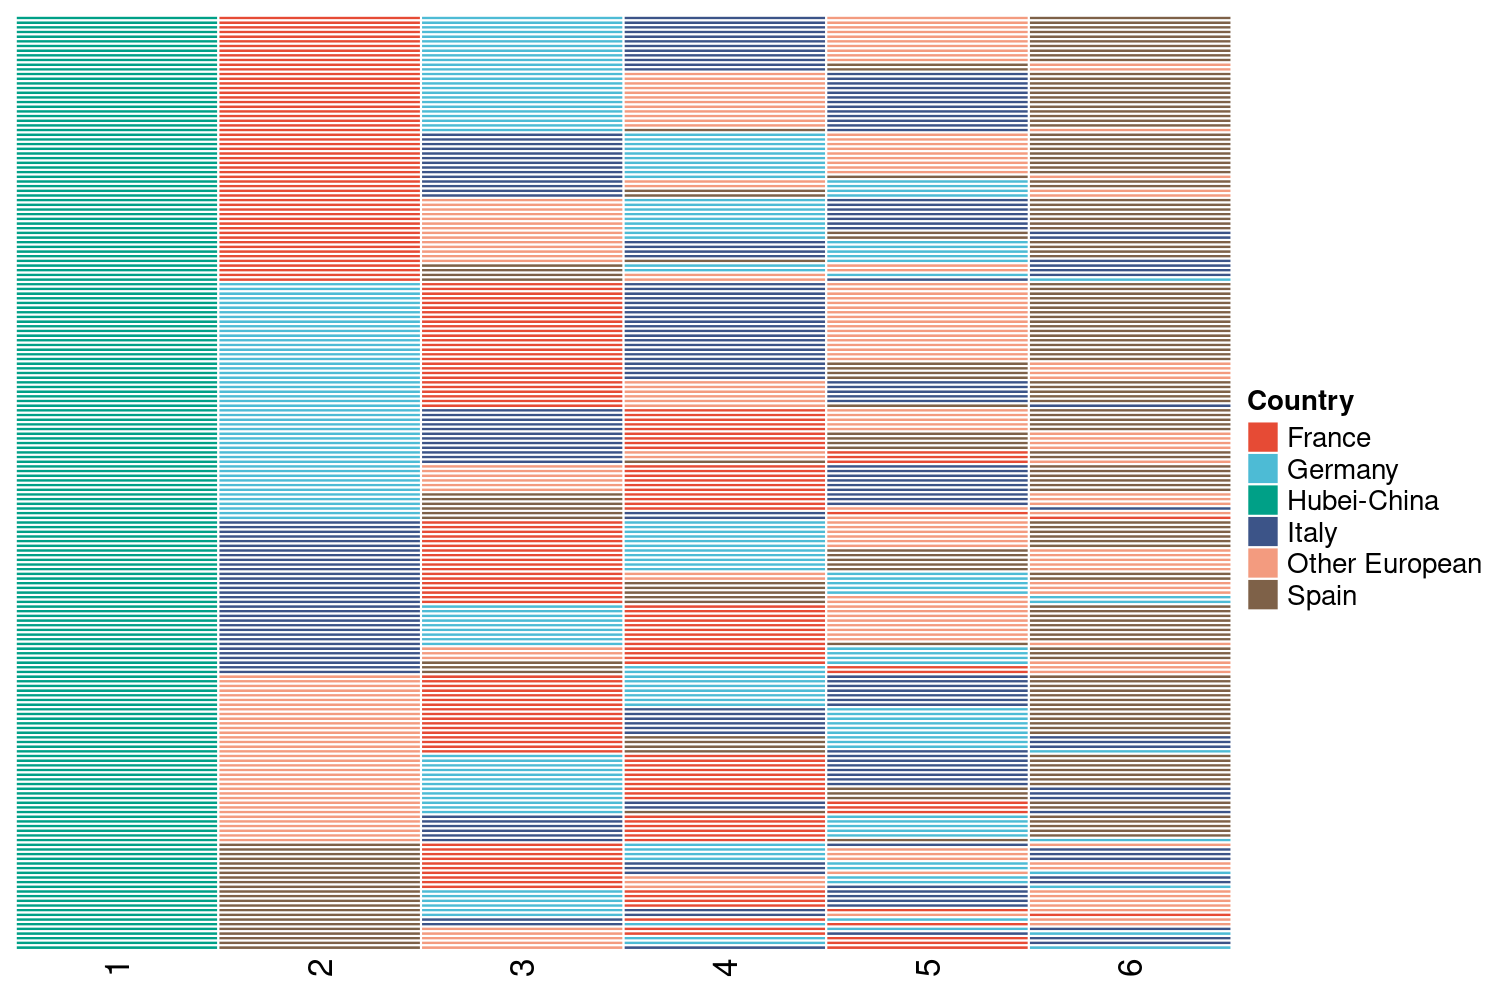
\includegraphics[width=\textwidth]{201030_europe3_figtraj05.png}
    \caption{Order of countries by the time of its first introduction, i.e. first case in the country. Each row is the order for one of the subsampled epidemic trajectories and each column represents the position relative to the other countries first introduction, e.g. in first position for all epidemic trajectories is China since it is the origin of the epidemic.} 
    \label{fig:first_imig}
\end{figure}

Along the same lines, we could ask if this order of countries is mantained when instead of looking at the first case in the country we look into at first case exported (migration) from that country to other European country. In Figure \ref{fig:first_omig} we observe a similar pattern to the first cases order, with Germany, France and Italy being the countries in the first positions in more than half of the inferred trajectories and never in the last position, and Spain as the country in last position in almost every epidemic trajectory.\\

\begin{figure}[ht]
    \centering
    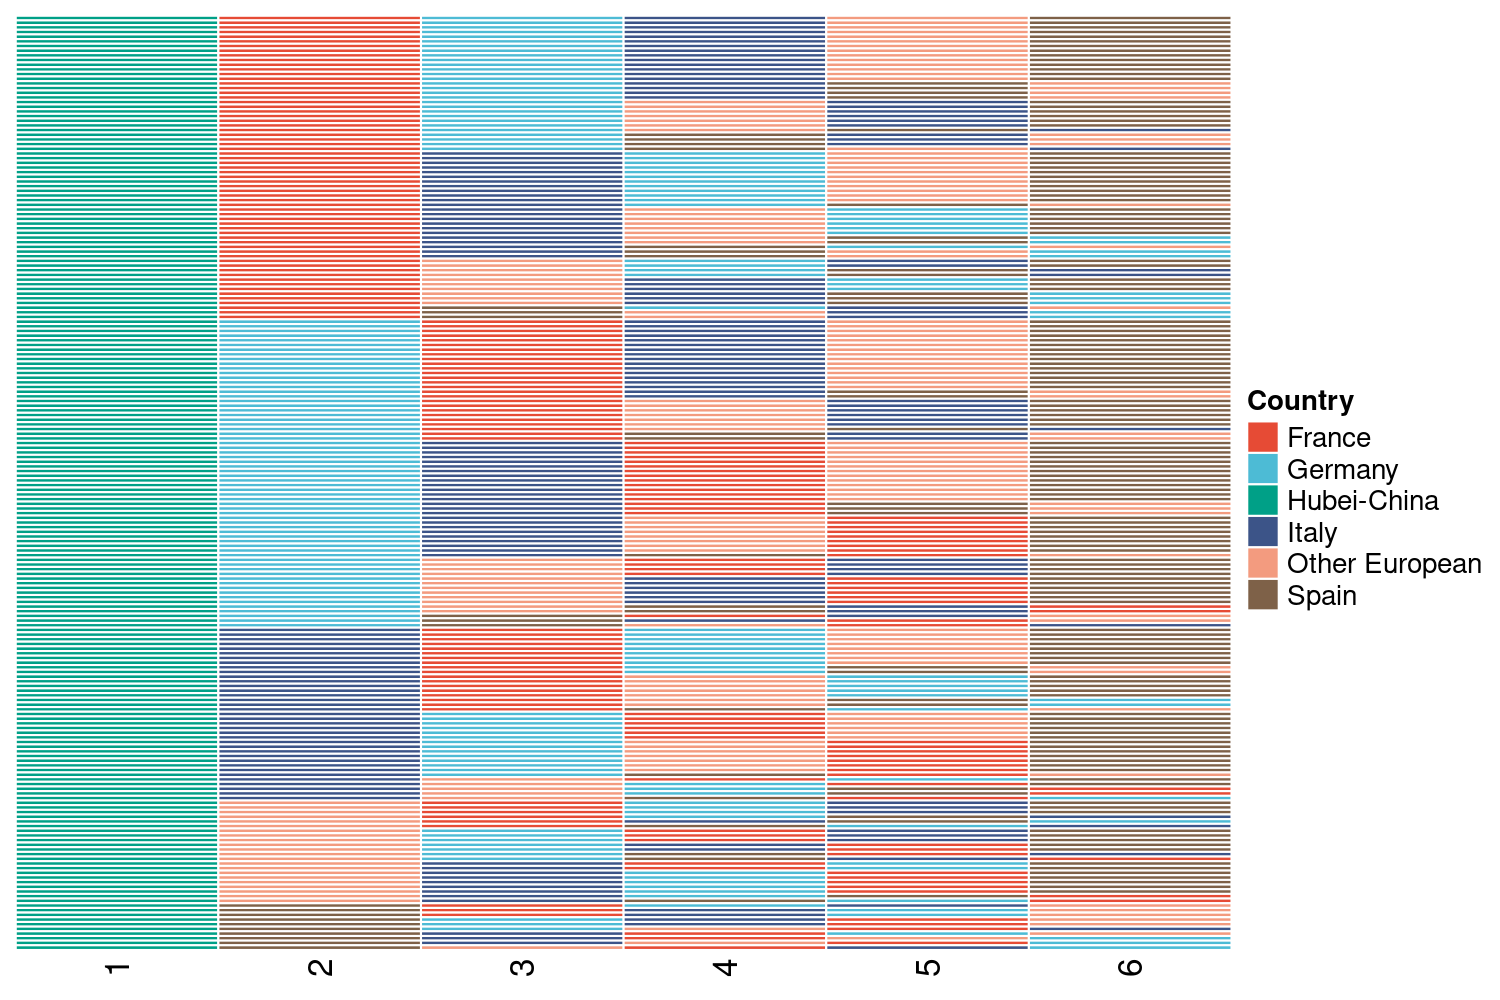
\includegraphics[width=\textwidth]{201030_europe3_figtraj06.png}
    \caption{Order of countries by the time of its first migration out of the country, i.e. first exported case to other country. Each row is the order for one of the subsampled epidemic trajectories and each column represents the position relative to the other countries first migration, e.g. in first position for all epidemic trajectories is China since it was the first country with exported cases of SARS-CoV-2 to other regions.}
    \label{fig:first_omig}
    \todo[inline]{I don't like much these "order" plots but maybe they could be useful to detect interesting patterns?}
\end{figure}

\subsubsection*{Migration vs within-region transmission}

\begin{figure}[ht]
    \centering
    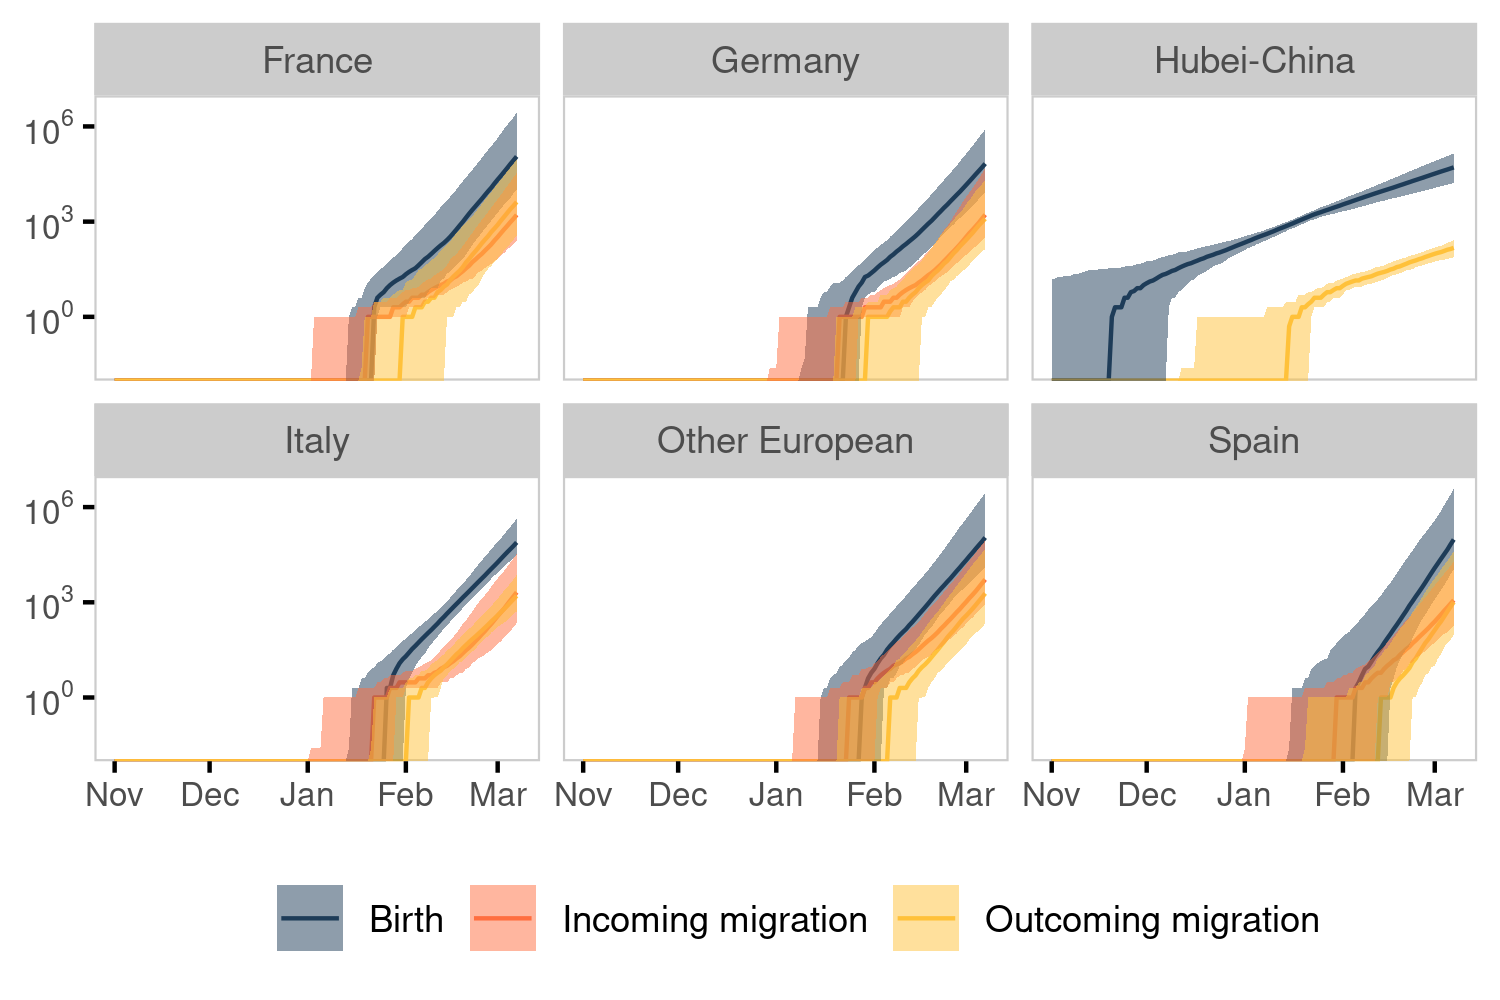
\includegraphics[width=\textwidth]{201030_europe3_figtraj07.png}
    \caption{Median and 95\% credible interval for the cumulative number of events (within-region transmissions and migrations to the country (incoming) and from the country (outgoing) over time.}
    \label{fig:events}
    \todo[inline]{change legend outgoing migration}
\end{figure}


\todo[inline]{TODO}

From the epidemic trajectories, we can extract the information about how many cases are within-region transmission and how many are migrations from other countries. The cumulative number of transmission events and migrations, represented in Figure \ref{fig:events} increases exponentially over time. An incomming migration into every European deme happens always before within-region transmission, seeding the epidemic. Within-region transmision accounts for most of the cases in the countries from late january onwards (when first cases were being reported in Europe).

\todo{get the proportion of within-region transmission and incoming migrations?}

The time between the first case in the country, i.e. first incoming migration event and the first case from within-region transmission is of x  (y-z) with similar values for all demes?. The time from the first incoming migration to the first outgoing migration is longer with a median of x (y-z). (This could be interesting to say if we should focus or not the screening and testing capacities to detect incoming migrations or if when we have evidence of cases in the population we shoud follow a more general strategy to find cases in the population according to the model. Is it different for each country?)\\

(How well did the countries detecting the first cases, there were already within region transmision?) We compare the date of the first reported rate of each country with the date in which within-region transmission for that country started according to the model. We see some differences among countries, France and Germany had in all inferred epidemic trajectories ongoing within-region transmission when first cases werre reported, while x\% of epidemic trajectories did not have had a within region transmission case when the first case in Spain was reported.\\

We can also compare the date of the first reported case with the date of the first outgoing migration from the country. (This could be interesting to say if a extreme measure closing borders with the first case could be effective to impede transmission to other countries: percentage of trajectories whre transmission to Europe would have been avoided. For other countries we can look at how many migrations events could have been avoided (and how many not) if the country closed borders after first reported case according to the model. Not realistic measure, extreme case.)\\ 



\subsubsection*{Migrations patterns}
Figures \ref{fig:migs_srcdest} and \ref{fig:migs}.\\
\todo[inline]{TODO}

Similar information in both plots, but in the chord plots instead of a daily evolution the time period is split on three (as in the GLM analysis). Chord plots are nicer and easier to understand I think, but barplots shows the great detail of the results of the model. Another advantage of the chrod plot is that the it shows mean absolute values and not only relative values.\\

Hubei-China is the majority source of migrations for all countries till February and then some patterns emerge (we expect more interesting results with the added info in GLM analysis).\\


\begin{figure}[!tbp]
  \centering

  \begin{minipage}[t]{0.4\textwidth}
  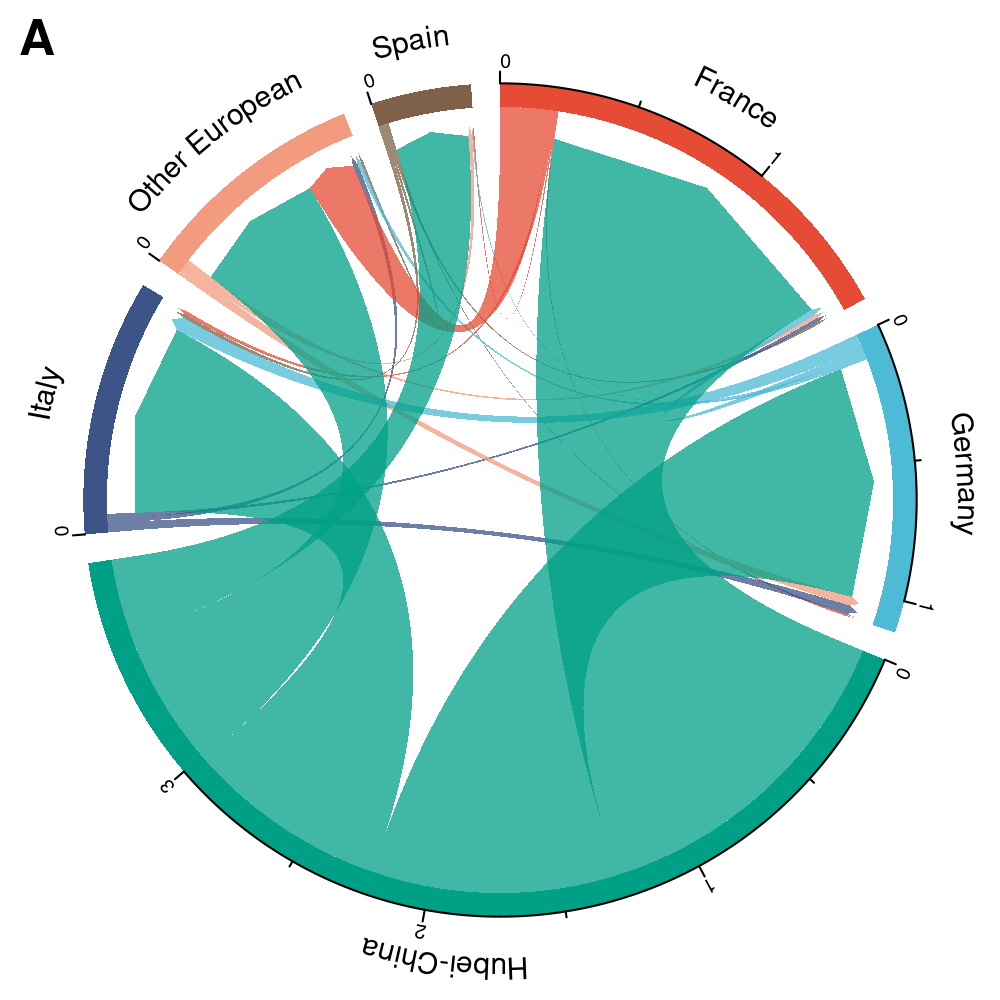
\includegraphics[width=\textwidth]{201030_europe3_figtraj09a.png}
  \label{fig:migs1}
  \end{minipage}
  \begin{minipage}[t]{0.4\textwidth}
  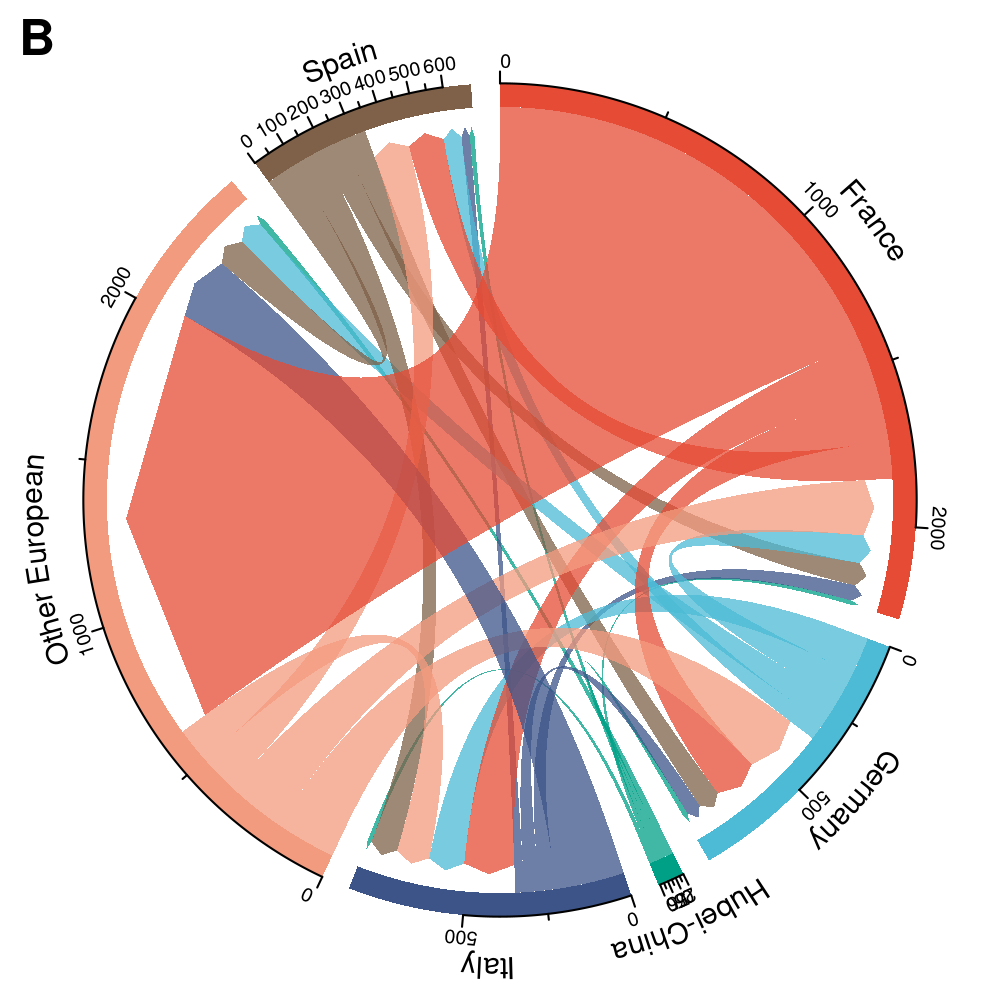
\includegraphics[width=\textwidth]{201030_europe3_figtraj09b.png}
  \label{fig:migs2}
  \end{minipage}
  \begin{minipage}[t]{0.4\textwidth}
  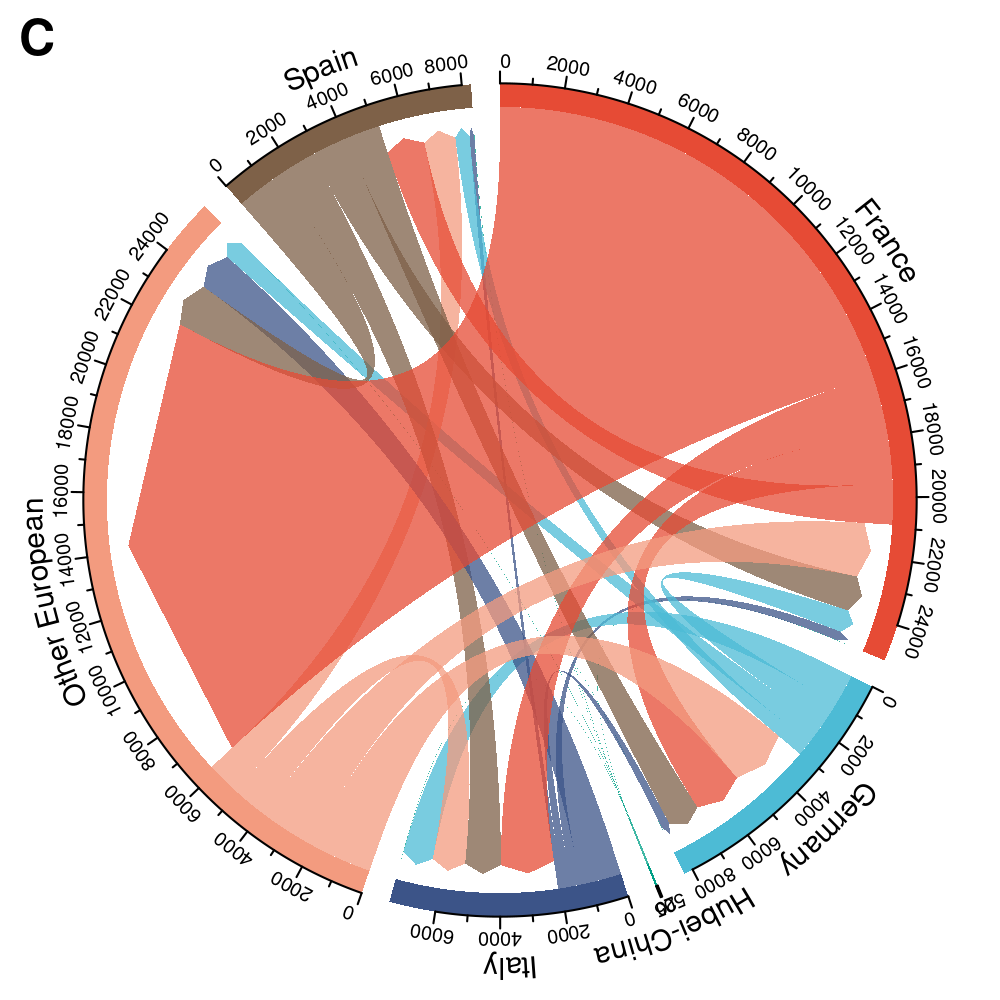
\includegraphics[width=\textwidth]{201030_europe3_figtraj09c.png}
  \label{fig:migs3}
  \end{minipage}
  \caption{Migration flux among demes over the three periods defined in the analysis.}
  \label{fig:migs}
\end{figure}

\begin{figure}[]
    \centering
    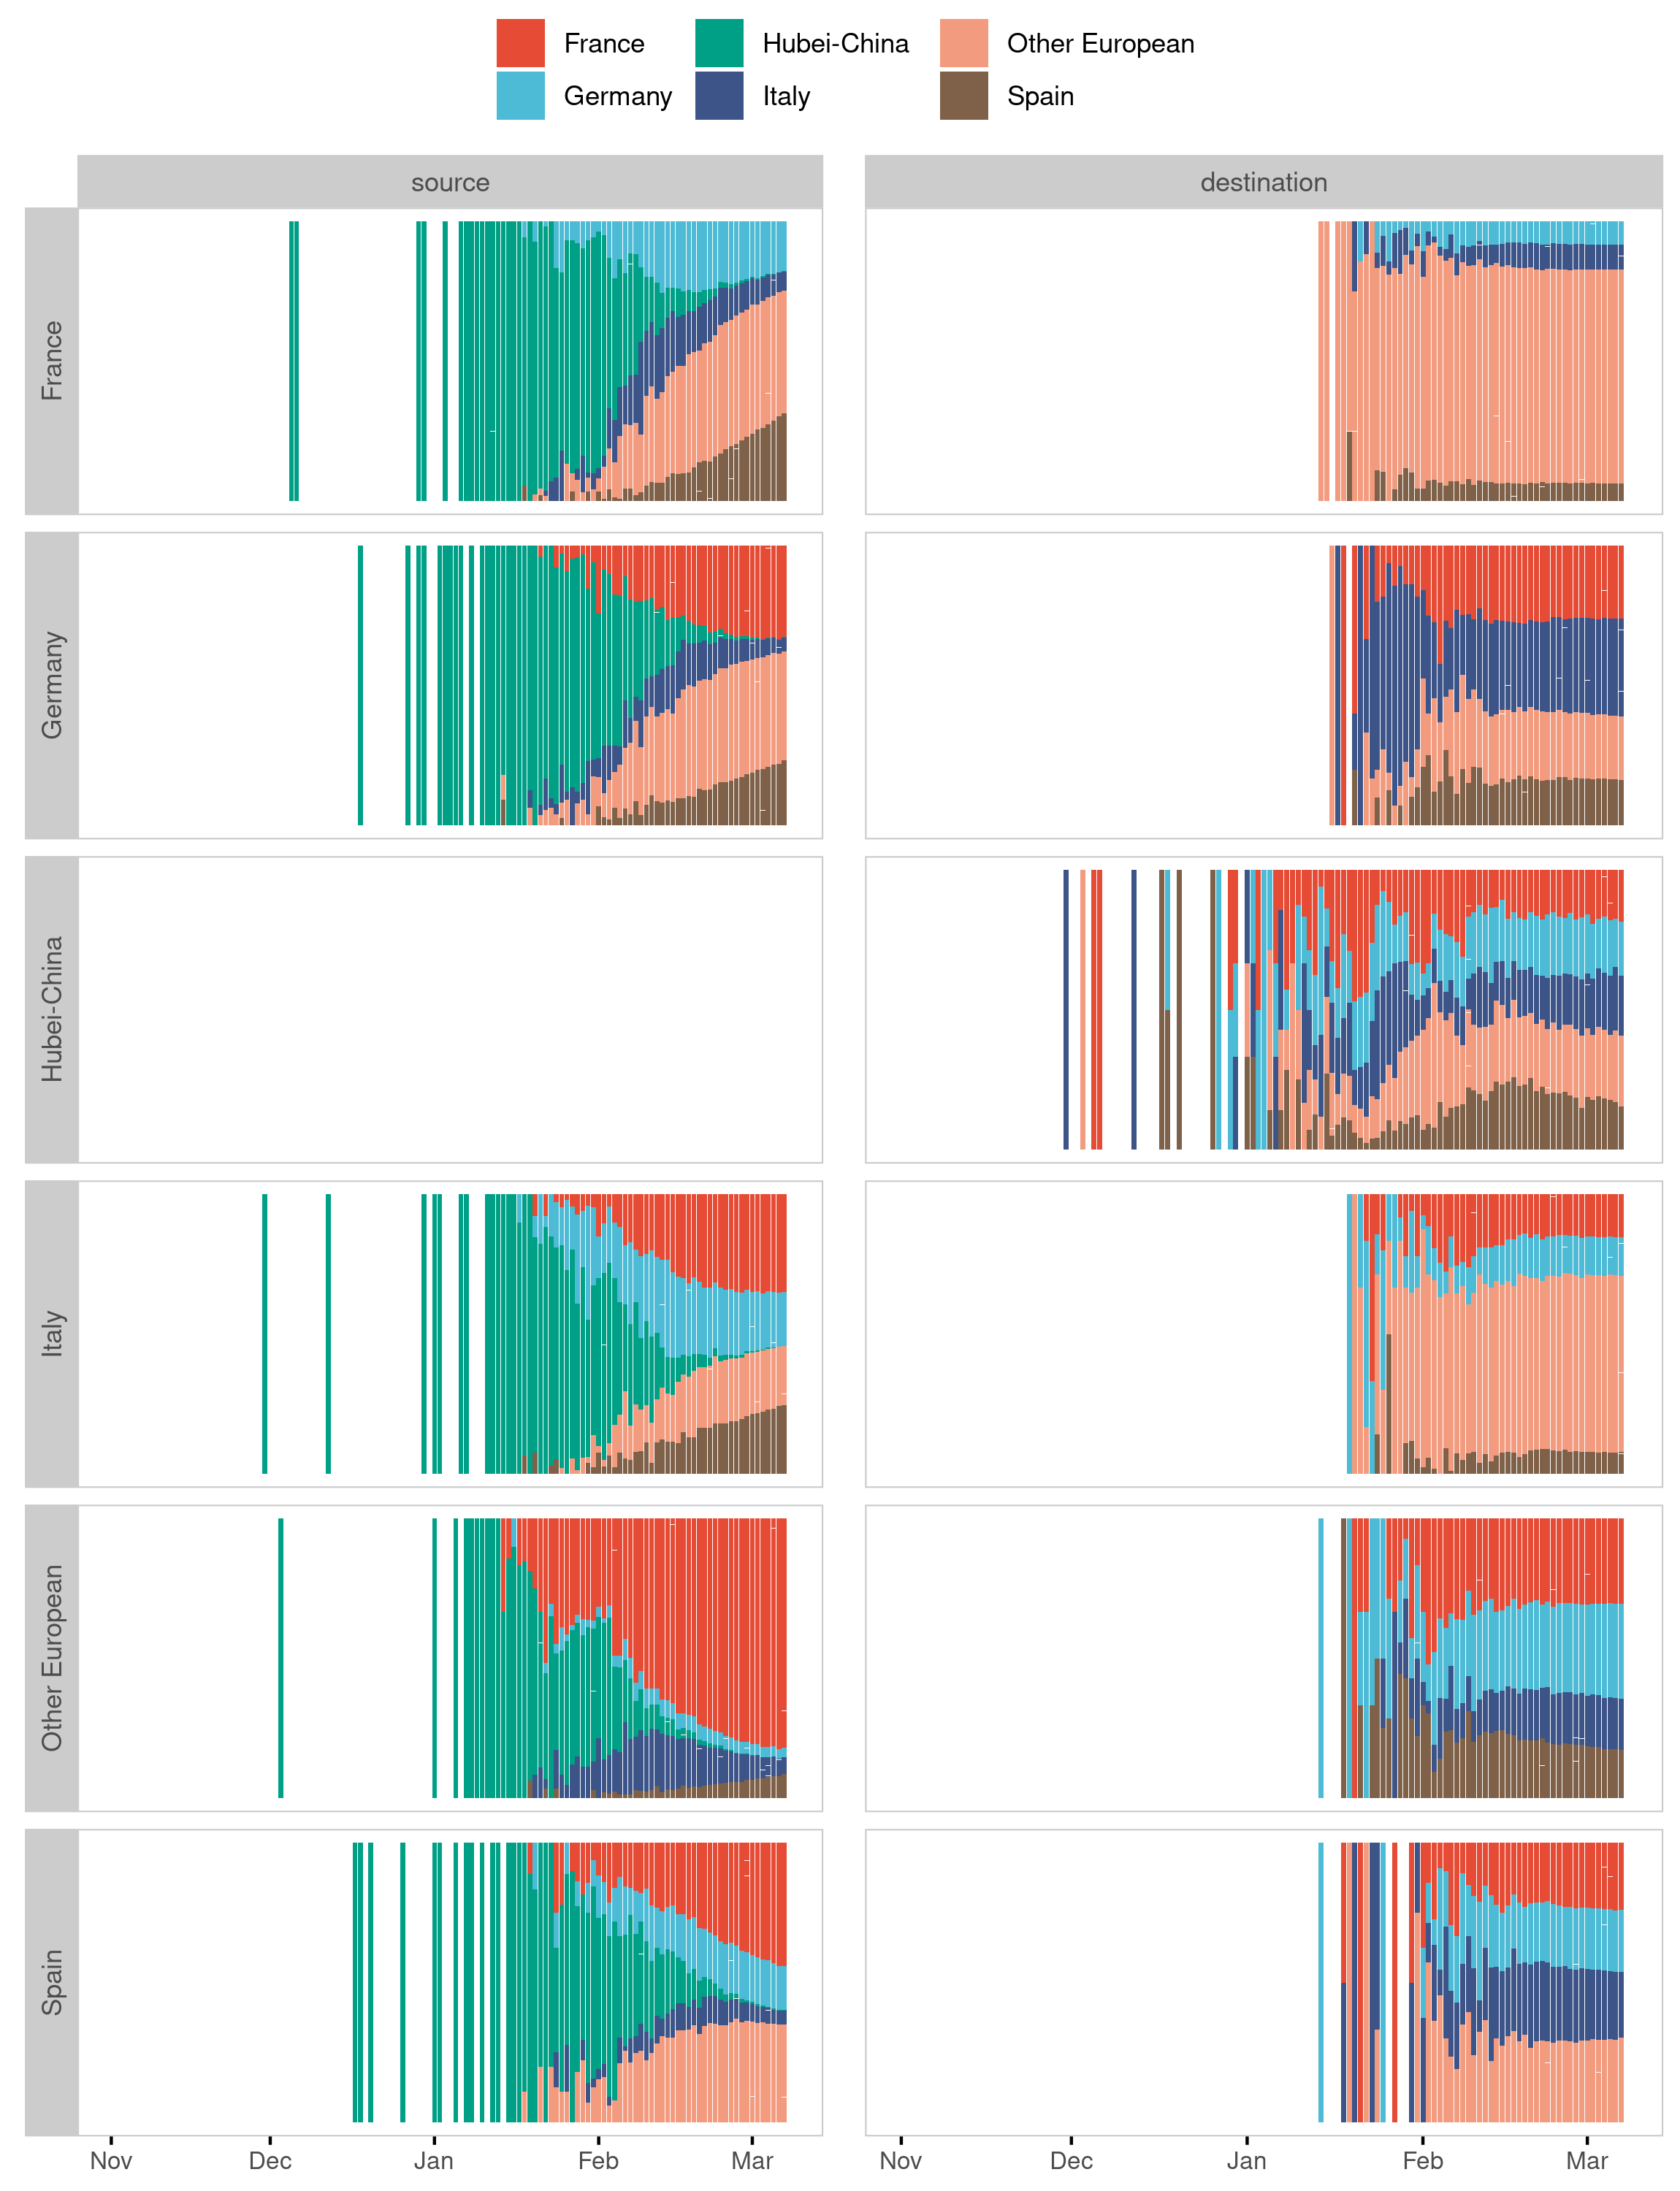
\includegraphics[width=\textwidth]{201030_europe3_figtraj08.png}
    \caption{}
    \label{fig:migs_srcdest}
\end{figure}


\subsubsection*{GLM predictors}
\todo[inline]{TODO}

Which channels were the main sources of transmission across national borders.

\subsubsection*{Epidemiological parameters}
\todo[inline]{TODO}

Not sure if it is necessary. But maybe include, briefly, the values of estimate R0, migration and sampling rates?


\section*{Discussion}
\todo[inline]{TODO discussion}

\begin{itemize}
\item Case counts discussion and reporting rates, second wave in Europe. Other estimations in other studies.

% Inferred population trajectories that account for all cases in the country. It is not an independent estimate since we are using informative priors for the sampling rates (upperbound computed as sequences/reported cases) and the subsampling scheme also includes the number of cases in the country (but that is a weaker link I think.\\


\item First introduction other studies. 

\item Migration patterns other studies.

\item Discuss assumptions of the model, caveats and possible improvements.
\end{itemize}

\section*{Conclusion}
\todo[inline]{TODO conclusion}

\section*{Material and Methods}
\todo[inline]{TODO methods}
\begin{itemize}
\item Dataset and subsampling. Alignment. 

\item Model BDMM-Prime, stochastic mapping. Priors. Bayesian phylogeographic inference. Phylodynamics.

\item GLM model. External data.

\item ?Same analysis but with travel data from last year, can we observe a consequence of Hubei lockdown and reduced travel?

\item Trajectories analysis. Subsampling and summarizing (median, 95\% interval)


\item Snakemake workflow.
\end{itemize}

\bibliographystyle{unsrt}
\bibliography{references-mt}

\listoftodos

\end{document}